\section{Problemstellung und Zielsetzung}\label{sec:definitionen}
\subsection{Das Problem der Weglauftendenz}\label{ssec:weglauftendenz}
Eine sogenannte Weglauftendenz, also die Neigung zum \enquote{Ausbüxen} von zu Hause oder aus der Pflegeeinrichtung, entwickeln sehr viele Demente Menschen. Oftmals gibt es einen Grund wie Langeweile oder das Gefühl, am falschen Ort zu sein. Patienten in einem Pflegeheim haben häufig die Idee, ihr Elternhaus oder die Arbeitsstelle aufzusuchen. Es wird unterschieden zwischen ziellosen Umherwandern (Rastlosigkeit) und zielgerichtetem Aufbrechen, weswegen oftmals das Wort \enquote{Hinlauftendenz} präferiert wird \citep[Vgl.][]{hinlauf}. Das Problem dabei ist, dass der Kranke in der Regel vergessen hat, warum oder wohin er eigentlich losgegangen ist \citep[Vgl.][]{dgk}. Dabei gehen die Patienten das Risiko der Dehydration, Unterzuckerung, oder unterbliebener Medikation ein. Im Winter besteht zudem Erfrierungsgefahr. In der Pflege von Menschen mit Weglauftendenz herrscht eine Spannung zwischen zwei sich widersprechenden Grundsätzen: Einerseits hat jeder Mensch das Recht, sich frei zu bewegen. Gleichzeitig sollen die dementen Menschen vor Gesundheitsgefahren beschützt werden \citep[Vgl.][]{pqsg}.
\subsection{Related Work: IoT-Anwendungen in Medizin und Pflege}\label{ssec:rel.work}
Das Welt des Internet of Things (IoT)) ist bereits auf die Pflege als lukratives Anwendungsfeld gestoßen.
\nomenclature{IoT}{\textbf{I}nternet \textbf{o}f \textbf{T}hings}
 Dementsprechend sind bereits einige Lösungen auf dem Markt, die durch die Nutzung von Technologien wie Bluetooth, GPS, Druck- und Beschleunigungssensoren versuchen, die Arbeit von Pflegenden zu erleichtern. Millionen von Sensoren, Aktoren, Mikrocontrollern und Kommunikationsgeräten erfassen rund um die Uhr Patientendaten, werten Muster und Auffälligkeiten aus und können so individuelle Versorgung, Diagnose oder Überwachung von pflegebedürftigen Menschen bereitstellen \citep[Vgl.][]{digikey}.
Das deutsche Bundesministerium für Bildung und Forschung (BMBF) hat eigens für die Weiterentwicklung solcher Themen eine Initiative mit dem Namen \enquote{Pflegeinnovationen 2020} ins Leben gerufen. Unter anderem werden durch diese Initiative Forschungsprojekte gefördert, die Innovationen der Mensch-Technik-Interaktion entwickeln und dadurch Pflegende unterstützen \citep[Vgl.][]{bmbf}. Fertige Produkte und Systeme sind bereits einige auf dem Markt.
Beispielsweise hat ein 13-Jähriger ein Überwachungssystem für seinen Großvater entwickelt, das in seine Socken integriert ist. Damit kann über Drucksensoren registriert werden, wann er nachts aufsteht \citep[Vgl.][]{spiegel-alzheimer}. Nach dem ähnlichen Prinzip funktionieren auch druckempflindliche Fußmatten, die schon weit verbreitet eingesetzt werden, beispielsweise als Bettvorleger oder am Zimmerausgang.  Ein Experiment der Intel-GE Care Innovations beispielsweise setzt den Fokus auf das \enquote{Altern vor Ort} und erforscht hierbei Technologien und Produkte, die es Senioren ermöglichen, so lange wie möglich selbständig zu Hause zu leben. Der erste Prototyp dieser Firma war der sogenannte \enquote{Magic Carpet} - ein mit Sensoren ausgestatteter Fußboden, der in der Wohnung einer älteren Person installiert werden kann. Zunächst werden typische Bewegungsmuster und Alltagsrituale über den Fußboden erfasst, wie zum Beispiel der Gang in die Küche jeden Morgen um 7 Uhr. Anschließend wird das Verhalten der Person regelmäßig auf Abnormalitäten überprüft. Bei einer kritischen Abweichung werden Angehörige oder Ärzte informiert \citep[Vgl.][S.49]{bigdata}.\\
Auch Wearables, also am Körper tragbare elektronische Helfer, sind bereits im Pflege-Bereich angekommen. Die Firma Eurotronik bietet beispielsweise ein System an, bei dem Demente mit Weglauftendenz über ein Funk-Armband geortet werden können. Zudem wird ein Alarm ausgelöst, wenn sie ihre erlaubten Aufenthaltsbereiche verlassen \citep[Vgl.][]{eurotronik}. Etwas diskreter ist der Einsatz von GPS-Armbanduhren. Diese werden von den Patienten nicht unbedingt als Ortungsarmband erkannt, was eine gesteigerte Benutzerakzeptanz nach sich zieht. Ein Beispiel hierfür sind die Uhren der Firma DS Vega \citep[Vgl.][]{ds-vega}.
Einen ähnlichen Ansatz der Ortung hat die Firma Aetrex gewählt, die einen GPS-Tracker unauffällig in spezielle Schuhe einbaut. Die Schuhe senden alle 30 Minuten die Position des Trägers an einen Account, den die Angehörigen oder die Pfleger einsehen können. Die Akkulaufzeit der GPS-Sender beträgt allerdings maximal 48 Stunden \citep[Vgl.][]{aetrex}.

\nomenclature{GPS}{\textbf{G}lobal \textbf{P}ositioning \textbf{S}ystem}
\nomenclature{BMBF}{\textbf{B}undes\textbf{m}inisterium für \textbf{B}ildung und \textbf{F}orschung}


\subsection{Projektübersicht iCare}
Das Projekt iCare ist ein vor einigen Jahren als Wettbewerbsidee ins Leben gerufenes Projekt mit dem Ziel, Menschen das \enquote{Altern zu Hause} zu ermöglichen und dabei Angehörige und Pfleger zu unterstützen.  Das iCare-Projekt ist über die studentische Projektarbeit hinaus bereits ein von der internationalen Bodenseehochschule gefördertes Forschungsprojekt \citep[Vgl.][]{icare-dhbw}. Eine Projektübersicht befindet sich in Anhang \ref{anh:icare}.
Das DeSearch-System als ein Teil von iCare beschäftigt sich mit der selben Problemstellung wie die bereits in Kapitel \ref{ssec:rel.work} erwähnten Systeme: Demente Personen mit Weglauftendenz. Allerdings soll das Ortungssystem von DeSearch dabei nicht vom Patienten erkannt werden. Ein Armband oder eine GPS-Uhr trägt immer das Risiko, von der dementen Person als eine Art \enquote{elektronische Fußfessel} angesehen zu werden. Sobald die Person die Uhr oder das Armband abnimmt, ist das System außer Kraft gesetzt. Einige Hersteller lösen dieses Problem mit Verschlüssen, die abgeschlossen werden können oder nur mit 2 Händen geöffnet werden können. Doch auch solche Systeme kann ein Patient zerstören, wenn er nicht mit der Ortung einverstanden ist. Beispielsweise steigen die Patienten dann mit dem Armband in die Badewanne oder greifen zu Scheren oder Messern, um die unerwünschten Geräte loszuwerden. Das Problem der Nutzerakzeptanz soll beim DeSearch-System dadurch gelöst werden, dass die Bluetooth-Marken, die zur Ortung dienen, unsichtbar in die Kleidung der Patienten eingenäht werden können. Auch wasserdicht und waschmaschinenfest sollen die Marken sein, sodass sie einfach mit der Kleidung mitgewaschen werden können. Ein weiteres Problem von GPS-Tracking-Systemen ist die Akkulaufzeit der Geräte. Die GPS-Schuhe müssen alle 48 Stunden geladen werden, die GPS-Uhr hat eine maximale Akkulaufzeit von 72 Stunden, abhängig von der Mobilfunknetz-Abdeckung. Mit der Auswahl von Bluetooth als Technologie für die Ortung haben die DeSearch-Marken den Vorteil, dass sie deutlich länger mit einer kleinen Knopfzelle betrieben werden können. Der Bluetooth-Low-Energy Standard ist hierfür maßgeblich (siehe Kapitel \ref{sssec:BLE}).

\subsection{Zielsetzung}
Das übergeordnete Ziel von iCare ist es, alternden Menschen so lange wie möglich das Leben zu Hause in einer vertrauten Umgebung zu bieten. Durch innovative Technologien, die Vernetzung von Geräten und Computerprogramme soll dieses Ziel verwirklicht werden und den Pflegern die Arbeit erleichtert werden. Ein Teil davon ist das DeSearch-System, das demente Patienten mit einer Weglauftendenz schützen und den Angehörigen oder Pflegern bei der Betreuung helfen soll.
Zielsetzung des DeSearch-Projektes ist die Entwicklung eines Ortungssystems, das von den Patienten unbemerkt in die Kleidung eingenäht wird. Die Anschaffungskosten sollen im Vergleich zu bisher auf dem Markt existenten Systemen niedrig sein, damit möglichst viele Kleidungsstücke mit Marken ausgestattet werden soll. Die Ortung von vermissten Personen soll über die Bluetooth-Low-Energy Technologie realisiert werden, damit die Marken eine möglichst lange Akkulaufzeit erreichen. Zudem darf die Position der Personen nicht dauerhaft aufgezeichnet werden, sondern nur im Vermisstenfall einmalig ermittelt werden. Eine Speicherung der Aufenthaltsorte wird nicht vorgenommen. Die Ortung erfolgt über eine Erkennung der Bluetooth-Marken von sogenannten DeSearch-Boxen, die in der Umgebung installiert werden. Diese melden den Fund dann an eine Zentrale, die die Ergebnisse auf einer Web-Oberfläche darstellt. Eine schematische Übersicht über die Funktionsweise von DeSearch ist in Abbildung \ref{fig:desearch} zu sehen. 
\begin{figure}
	\centering
	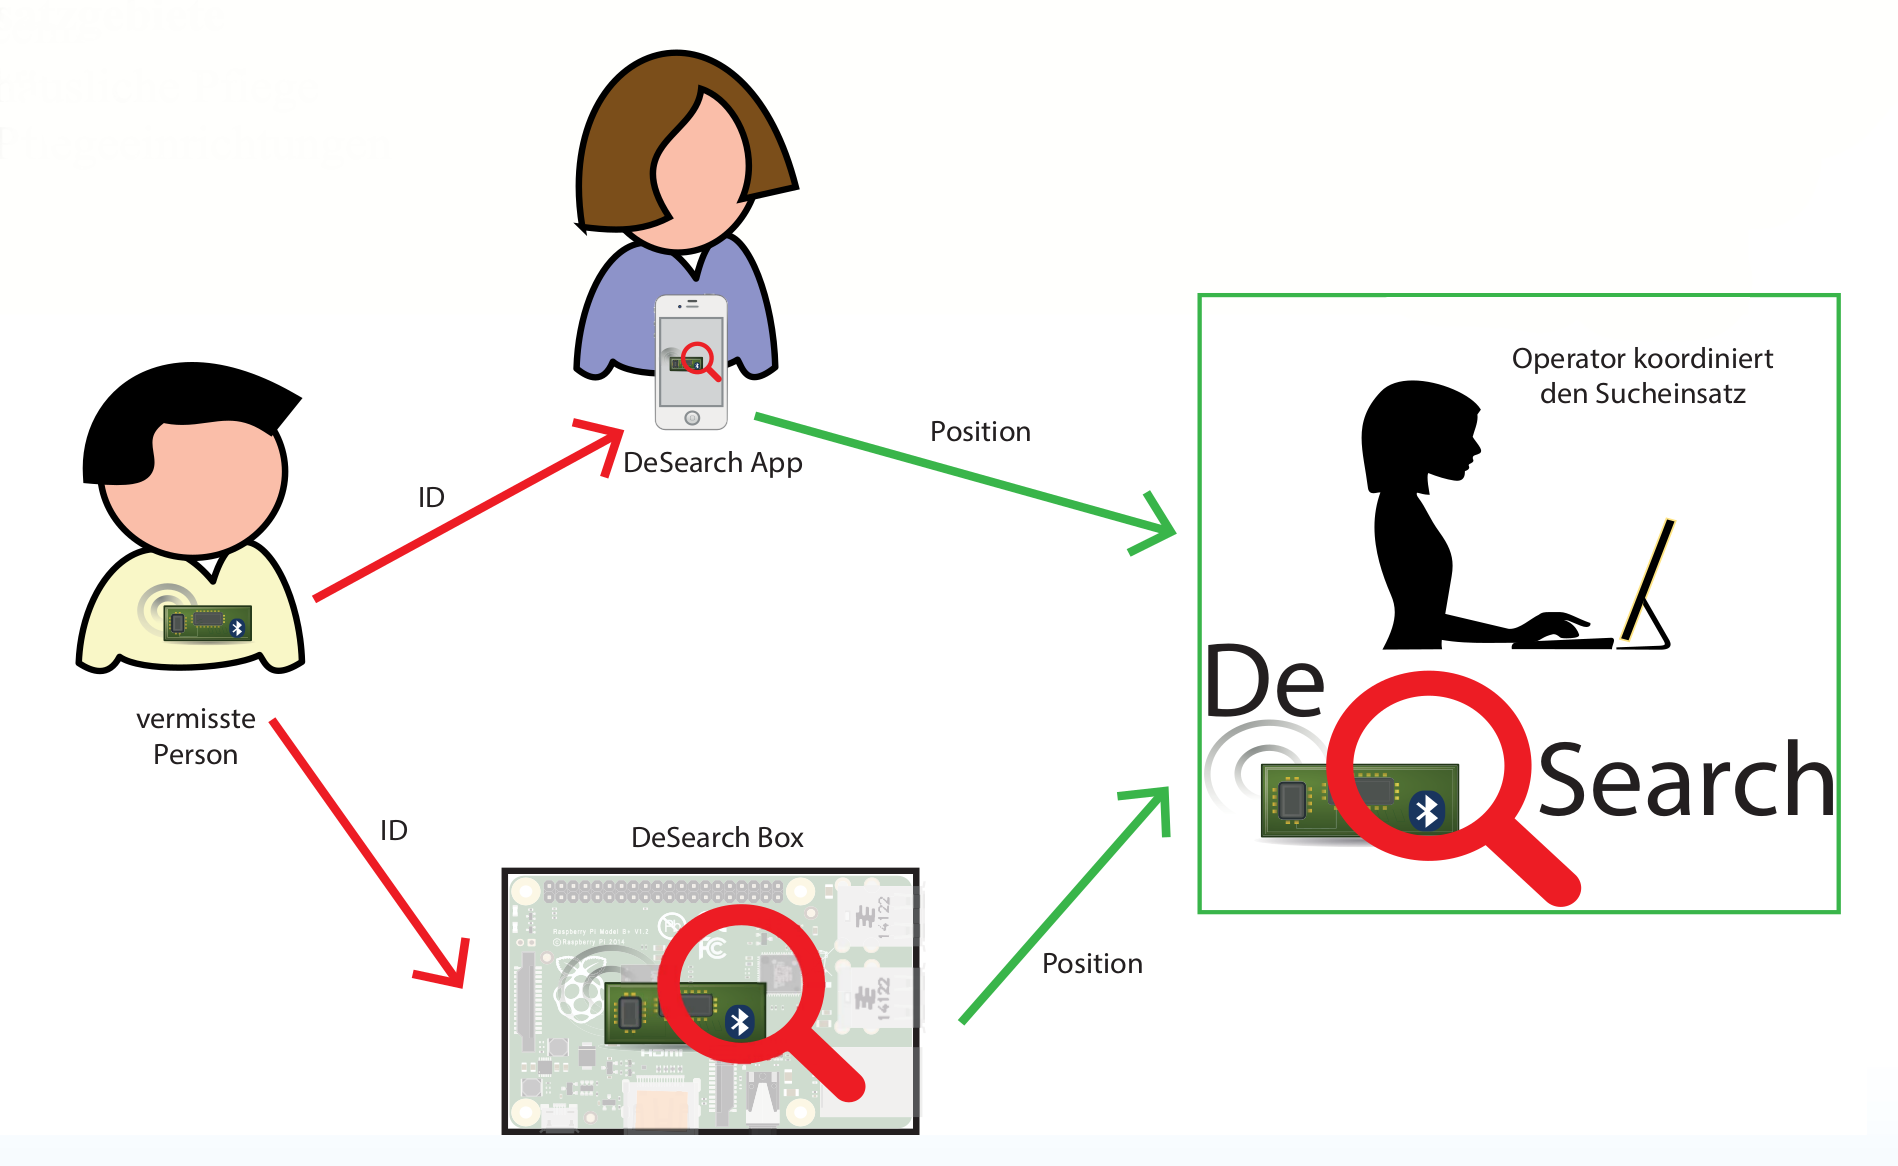
\includegraphics[width=\textwidth]{images/iCare-Systematik}
	\caption[Funktionsweise des DeSearch-Systems]{Schematische Darstellung der Funktionsweise des DeSearch-Systems, Quelle: http://www.bodenseehochschule.org/wp-content/uploads/2015/12/IBH\_ProjektPlakate\_A0\_iCare.pdf }
	\label{fig:desearch}
\end{figure} 
Im Rahmen dieser Projektarbeit soll ein lauffähiger Prototyp der Zentrale, der DeSearch-Boxen und der Web-Oberfläche erstellt werden, der dann in einer Testumgebung an der dualen Hochschule getestet werden soll.
